\begin{frame}{Text editors}
  \begin{columns}[T]
    \begin{column}{0.45\textwidth}
      \textbf{TextWrangler}
      \begin{itemize}
      \item An informal survey indicates -
        9 out of 10 iPQB students using OSX think that TextWrangler
        is a better text editor than Crest toothpaste
      \item Also, it should be installed on your laptop
      \end{itemize}
      \begin{center}
        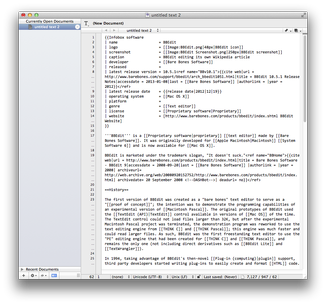
\includegraphics[keepaspectratio=true,width=0.45\textwidth]
        {figures/BBEdit-Screenshot.png}        
      \end{center}
    \end{column}
    \begin{column}{0.45\textwidth}
      \textbf{PyCharm}
      \begin{itemize}
      \item PyCharm is a Python-focused
        \href{http://en.wikipedia.org/wiki/Integrated_development_environment}{IDE}
        - a text editor combined with a debugger and other powerful
        features to help with \textit{serious} development
      \item Useful if you are writing large Python applications
      \end{itemize}
      \begin{center}
        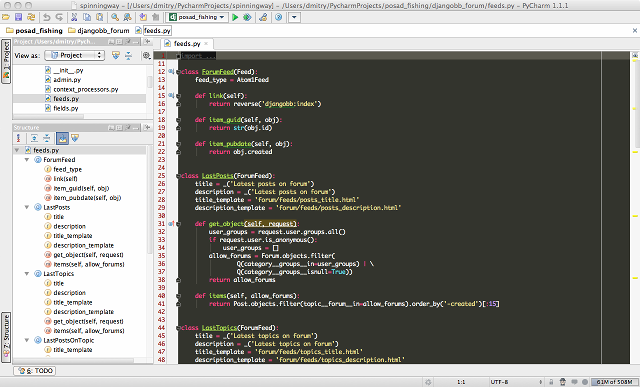
\includegraphics[keepaspectratio=true,width=0.45\textwidth]
        {figures/pycharm-screenshot.jpg}
      \end{center}
    \end{column}
  \end{columns}
\end{frame}

\begin{frame}{\textit{Real} text editors}
  There are only two choices - Emacs or Vim
  \begin{itemize}
  \item Both are cross-platform and can be used on any OS
  \item Both support syntax highlighting for pretty much anything
    \pause
  \item There are disagreements as to which one is better...
  \end{itemize}
  \begin{center}
    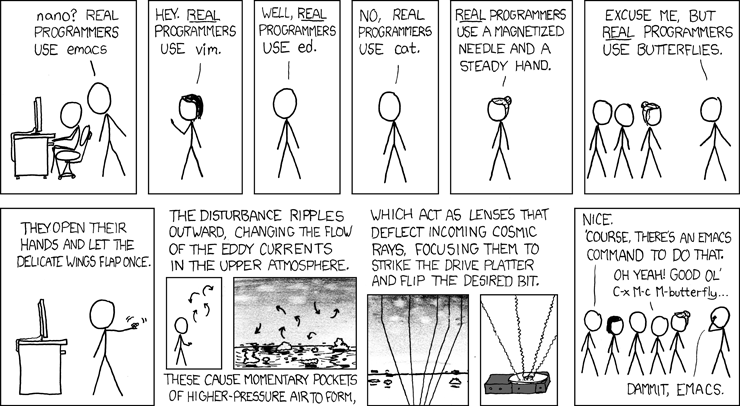
\includegraphics[keepaspectratio=true,width=0.85\textwidth]
    {figures/real-programmers.png}
  \end{center}
  {\tiny - Citation - \href{http://xkcd.com/378/}{XKCD 378}}
\end{frame}